\documentclass[twoside]{book}

% Packages required by doxygen
\usepackage{calc}
\usepackage{doxygen}
\usepackage{graphicx}
\usepackage[utf8]{inputenc}
\usepackage{makeidx}
\usepackage{multicol}
\usepackage{multirow}
\usepackage{textcomp}
\usepackage[table]{xcolor}

% Font selection
\usepackage[T1]{fontenc}
\usepackage{mathptmx}
\usepackage[scaled=.90]{helvet}
\usepackage{courier}
\usepackage{amssymb}
\usepackage{sectsty}
\renewcommand{\familydefault}{\sfdefault}
\allsectionsfont{%
  \fontseries{bc}\selectfont%
  \color{darkgray}%
}
\renewcommand{\DoxyLabelFont}{%
  \fontseries{bc}\selectfont%
  \color{darkgray}%
}

% Page & text layout
\usepackage{geometry}
\geometry{%
  a4paper,%
  top=2.5cm,%
  bottom=2.5cm,%
  left=2.5cm,%
  right=2.5cm%
}
\tolerance=750
\hfuzz=15pt
\hbadness=750
\setlength{\emergencystretch}{15pt}
\setlength{\parindent}{0cm}
\setlength{\parskip}{0.2cm}
\makeatletter
\renewcommand{\paragraph}{%
  \@startsection{paragraph}{4}{0ex}{-1.0ex}{1.0ex}{%
    \normalfont\normalsize\bfseries\SS@parafont%
  }%
}
\renewcommand{\subparagraph}{%
  \@startsection{subparagraph}{5}{0ex}{-1.0ex}{1.0ex}{%
    \normalfont\normalsize\bfseries\SS@subparafont%
  }%
}
\makeatother

% Headers & footers
\usepackage{fancyhdr}
\pagestyle{fancyplain}
\fancyhead[LE]{\fancyplain{}{\bfseries\thepage}}
\fancyhead[CE]{\fancyplain{}{}}
\fancyhead[RE]{\fancyplain{}{\bfseries\leftmark}}
\fancyhead[LO]{\fancyplain{}{\bfseries\rightmark}}
\fancyhead[CO]{\fancyplain{}{}}
\fancyhead[RO]{\fancyplain{}{\bfseries\thepage}}
\fancyfoot[LE]{\fancyplain{}{}}
\fancyfoot[CE]{\fancyplain{}{}}
\fancyfoot[RE]{\fancyplain{}{\bfseries\scriptsize Generated on Tue Mar 15 2016 13\-:11\-:03 for Actividad 3 by Doxygen }}
\fancyfoot[LO]{\fancyplain{}{\bfseries\scriptsize Generated on Tue Mar 15 2016 13\-:11\-:03 for Actividad 3 by Doxygen }}
\fancyfoot[CO]{\fancyplain{}{}}
\fancyfoot[RO]{\fancyplain{}{}}
\renewcommand{\footrulewidth}{0.4pt}
\renewcommand{\chaptermark}[1]{%
  \markboth{#1}{}%
}
\renewcommand{\sectionmark}[1]{%
  \markright{\thesection\ #1}%
}

% Indices & bibliography
\usepackage{natbib}
\usepackage[titles]{tocloft}
\setcounter{tocdepth}{3}
\setcounter{secnumdepth}{5}
\makeindex

% Hyperlinks (required, but should be loaded last)
\usepackage{ifpdf}
\ifpdf
  \usepackage[pdftex,pagebackref=true]{hyperref}
\else
  \usepackage[ps2pdf,pagebackref=true]{hyperref}
\fi
\hypersetup{%
  colorlinks=true,%
  linkcolor=blue,%
  citecolor=blue,%
  unicode%
}

% Custom commands
\newcommand{\clearemptydoublepage}{%
  \newpage{\pagestyle{empty}\cleardoublepage}%
}


%===== C O N T E N T S =====

\begin{document}

% Titlepage & ToC
\hypersetup{pageanchor=false}
\pagenumbering{roman}
\begin{titlepage}
\vspace*{7cm}
\begin{center}%
{\Large Actividad 3 }\\
\vspace*{1cm}
{\large Generated by Doxygen 1.8.6}\\
\vspace*{0.5cm}
{\small Tue Mar 15 2016 13:11:03}\\
\end{center}
\end{titlepage}
\clearemptydoublepage
\tableofcontents
\clearemptydoublepage
\pagenumbering{arabic}
\hypersetup{pageanchor=true}

%--- Begin generated contents ---
\chapter{cdi\-\_\-actividad\-\_\-3}
\label{md_README}
\hypertarget{md_README}{}
\subsection*{3.\-1 Un simple contador concurrente}

\subsubsection*{2. Elabora una clase \hyperlink{classContador}{Contador} que tiene un método Incrementar(n) que ejecuta un bucle de n iteraciones que incrementa una variable interna cada cierto tiempo, y al acabar devuelve el valor actual de dicha variable. Elabora un programa que lanza varios hilos que comparten tal objeto contador. Cada hilo, cada cierto tiempo, debe llamar al método Incrementar(n) con n adecuado e visualizar el valor devuelto por ese método. ¿\-Podemos garantizar que cuando un hilo ejecuta el método Incrementar() , no interferirá con otro hilo? ¿\-Cómo podemos solucionarlo (hay varias posibilidades)?}

No.\-Usando Synchronized o usando un join entre los threads, en este caso no seria concurrente.

\subsection*{3.\-2 Introducción a la sincronización de hilos}

\paragraph*{4. ¿\-Cuál es el resultado? ¿\-Cuántos hilos pueden estar simultáneamente ejecutando el método Enter\-And\-Wait()?}

Los hilos se inician en orden pero algunos de ellos pueden no finalizar en el mismo orden en el que se inicializaron. 
\chapter{Hierarchical Index}
\section{Class Hierarchy}
This inheritance list is sorted roughly, but not completely, alphabetically\-:\begin{DoxyCompactList}
\item \contentsline{section}{Actvidad3\-\_\-3}{\pageref{classActvidad3__3}}{}
\item \contentsline{section}{Contador}{\pageref{classContador}}{}
\item Runnable\begin{DoxyCompactList}
\item \contentsline{section}{Actividad3\-\_\-2}{\pageref{classActividad3__2}}{}
\item \contentsline{section}{B}{\pageref{classB}}{}
\end{DoxyCompactList}
\end{DoxyCompactList}

\chapter{Class Index}
\section{Class List}
Here are the classes, structs, unions and interfaces with brief descriptions\+:\begin{DoxyCompactList}
\item\contentsline{section}{\hyperlink{classActividad3__2}{Actividad3\+\_\+2} \\*Resuelve la actividad 3.\+2 }{\pageref{classActividad3__2}}{}
\item\contentsline{section}{\hyperlink{classContador}{Contador} \\*Implementa uncontador }{\pageref{classContador}}{}
\end{DoxyCompactList}

\chapter{File Index}
\section{File List}
Here is a list of all files with brief descriptions\+:\begin{DoxyCompactList}
\item\contentsline{section}{src/\hyperlink{Actividad3__2_8java}{Actividad3\+\_\+2.\+java} }{\pageref{Actividad3__2_8java}}{}
\item\contentsline{section}{src/\hyperlink{Contador_8java}{Contador.\+java} }{\pageref{Contador_8java}}{}
\end{DoxyCompactList}

\chapter{Class Documentation}
\hypertarget{classActividad3__2}{}\section{Actividad3\+\_\+2 Class Reference}
\label{classActividad3__2}\index{Actividad3\+\_\+2@{Actividad3\+\_\+2}}


Resuelve la actividad 3.\+2.  


Inheritance diagram for Actividad3\+\_\+2\+:\begin{figure}[H]
\begin{center}
\leavevmode
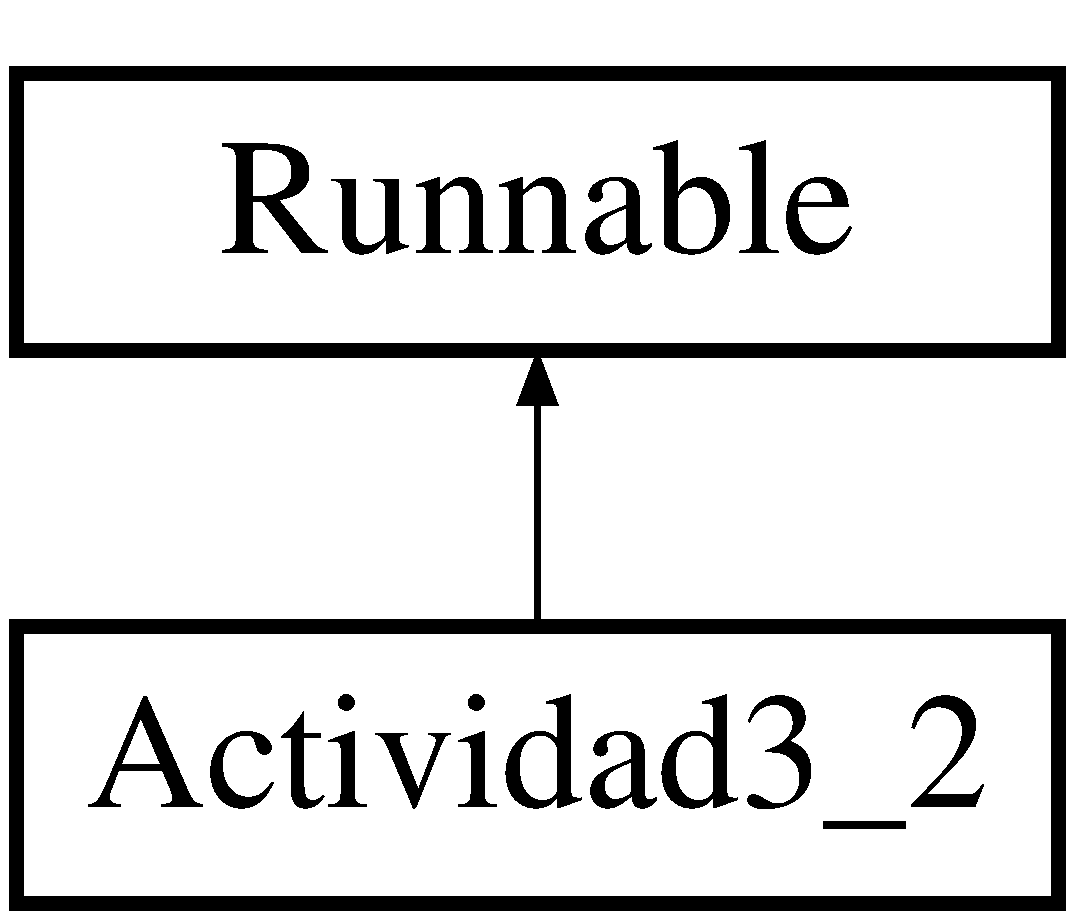
\includegraphics[height=2.000000cm]{classActividad3__2}
\end{center}
\end{figure}
\subsection*{Public Member Functions}
\begin{DoxyCompactItemize}
\item 
\hyperlink{classActividad3__2_a765178bf74270a5de1e36cfa9ae5d122}{Actividad3\+\_\+2} (int n)
\begin{DoxyCompactList}\small\item\em Constructor de la clase. \end{DoxyCompactList}\item 
void \hyperlink{classActividad3__2_abbd52976157c9a88e6308b9b336afd3d}{run} ()
\begin{DoxyCompactList}\small\item\em ejecuta el incremento indefinidamente \end{DoxyCompactList}\end{DoxyCompactItemize}
\subsection*{Static Public Member Functions}
\begin{DoxyCompactItemize}
\item 
static void \hyperlink{classActividad3__2_a1cde3718f03eb51c4a1180742170439f}{main} (String\mbox{[}$\,$\mbox{]} args)
\begin{DoxyCompactList}\small\item\em La funcion main crea y inicia 3 hilos con diferentes valores de incremento. \end{DoxyCompactList}\end{DoxyCompactItemize}


\subsection{Detailed Description}
Resuelve la actividad 3.\+2. 

\begin{DoxyAuthor}{Author}
vmfilgueira mmalvarez2 
\end{DoxyAuthor}


\subsection{Constructor \& Destructor Documentation}
\hypertarget{classActividad3__2_a765178bf74270a5de1e36cfa9ae5d122}{}\index{Actividad3\+\_\+2@{Actividad3\+\_\+2}!Actividad3\+\_\+2@{Actividad3\+\_\+2}}
\index{Actividad3\+\_\+2@{Actividad3\+\_\+2}!Actividad3\+\_\+2@{Actividad3\+\_\+2}}
\subsubsection[{Actividad3\+\_\+2}]{\setlength{\rightskip}{0pt plus 5cm}Actividad3\+\_\+2.\+Actividad3\+\_\+2 (
\begin{DoxyParamCaption}
\item[{int}]{n}
\end{DoxyParamCaption}
)}\label{classActividad3__2_a765178bf74270a5de1e36cfa9ae5d122}


Constructor de la clase. 


\begin{DoxyParams}{Parameters}
{\em n} & numero de incrementos \\
\hline
\end{DoxyParams}


\subsection{Member Function Documentation}
\hypertarget{classActividad3__2_a1cde3718f03eb51c4a1180742170439f}{}\index{Actividad3\+\_\+2@{Actividad3\+\_\+2}!main@{main}}
\index{main@{main}!Actividad3\+\_\+2@{Actividad3\+\_\+2}}
\subsubsection[{main}]{\setlength{\rightskip}{0pt plus 5cm}static void Actividad3\+\_\+2.\+main (
\begin{DoxyParamCaption}
\item[{String\mbox{[}$\,$\mbox{]}}]{args}
\end{DoxyParamCaption}
)\hspace{0.3cm}{\ttfamily [static]}}\label{classActividad3__2_a1cde3718f03eb51c4a1180742170439f}


La funcion main crea y inicia 3 hilos con diferentes valores de incremento. 


\begin{DoxyParams}{Parameters}
{\em args} & argumentos de la consola \\
\hline
\end{DoxyParams}
\hypertarget{classActividad3__2_abbd52976157c9a88e6308b9b336afd3d}{}\index{Actividad3\+\_\+2@{Actividad3\+\_\+2}!run@{run}}
\index{run@{run}!Actividad3\+\_\+2@{Actividad3\+\_\+2}}
\subsubsection[{run}]{\setlength{\rightskip}{0pt plus 5cm}void Actividad3\+\_\+2.\+run (
\begin{DoxyParamCaption}
{}
\end{DoxyParamCaption}
)}\label{classActividad3__2_abbd52976157c9a88e6308b9b336afd3d}


ejecuta el incremento indefinidamente 



The documentation for this class was generated from the following file\+:\begin{DoxyCompactItemize}
\item 
src/\hyperlink{Actividad3__2_8java}{Actividad3\+\_\+2.\+java}\end{DoxyCompactItemize}

\hypertarget{classActvidad3__3}{\section{Actvidad3\-\_\-3 Class Reference}
\label{classActvidad3__3}\index{Actvidad3\-\_\-3@{Actvidad3\-\_\-3}}
}


Resuelve la actividad 3.\-3.  


\subsection*{Static Public Member Functions}
\begin{DoxyCompactItemize}
\item 
static void \hyperlink{classActvidad3__3_adb7dc3bd5d6b9d9534217231cb488dcb}{main} (String\mbox{[}$\,$\mbox{]} args)
\begin{DoxyCompactList}\small\item\em Código princpal del programa. \end{DoxyCompactList}\end{DoxyCompactItemize}


\subsection{Detailed Description}
Resuelve la actividad 3.\-3. 

\subsection{Member Function Documentation}
\hypertarget{classActvidad3__3_adb7dc3bd5d6b9d9534217231cb488dcb}{\index{Actvidad3\-\_\-3@{Actvidad3\-\_\-3}!main@{main}}
\index{main@{main}!Actvidad3_3@{Actvidad3\-\_\-3}}
\subsubsection[{main}]{\setlength{\rightskip}{0pt plus 5cm}static void Actvidad3\-\_\-3.\-main (
\begin{DoxyParamCaption}
\item[{String\mbox{[}$\,$\mbox{]}}]{args}
\end{DoxyParamCaption}
)\hspace{0.3cm}{\ttfamily [static]}}}\label{classActvidad3__3_adb7dc3bd5d6b9d9534217231cb488dcb}


Código princpal del programa. 


\begin{DoxyParams}{Parameters}
{\em args} & Argumentos de la consola \\
\hline
\end{DoxyParams}


The documentation for this class was generated from the following file\-:\begin{DoxyCompactItemize}
\item 
src/\hyperlink{Actvidad3__3_8java}{Actvidad3\-\_\-3.\-java}\end{DoxyCompactItemize}

\hypertarget{classB}{\section{B Class Reference}
\label{classB}\index{B@{B}}
}


Clase \hyperlink{classB}{B} que se encarga de llamar a la clase A.  


Inheritance diagram for B\-:\begin{figure}[H]
\begin{center}
\leavevmode
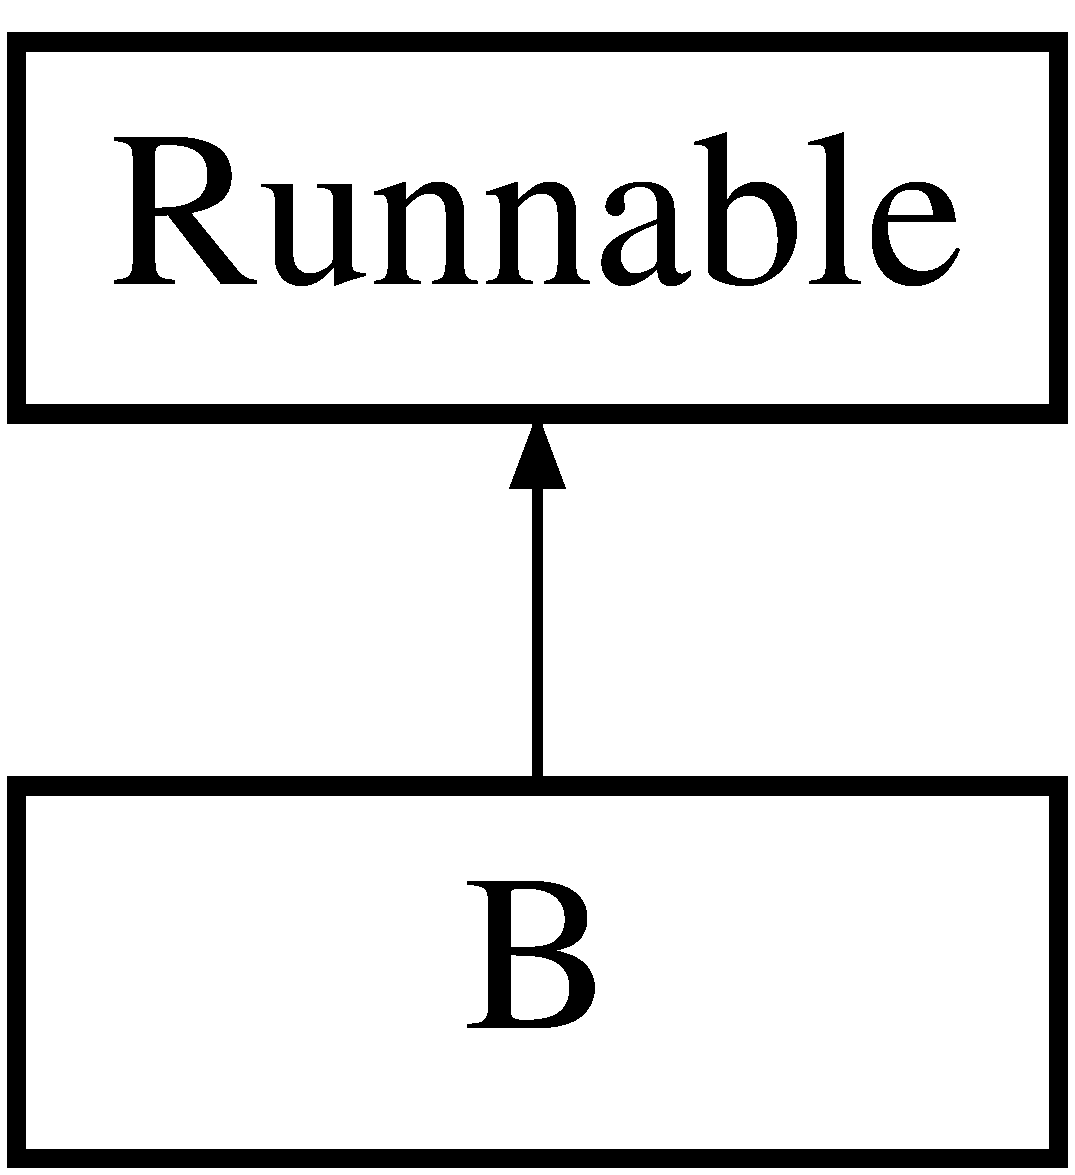
\includegraphics[height=2.000000cm]{classB}
\end{center}
\end{figure}
\subsection*{Public Member Functions}
\begin{DoxyCompactItemize}
\item 
\hyperlink{classB_a64880fe126d9d91e9b9226f56d0821ec}{B} (A a)
\begin{DoxyCompactList}\small\item\em Constructor que recibe un objeto de la clase A. \end{DoxyCompactList}\item 
void \hyperlink{classB_aba92474eb47bc61bfa0f239a750d090a}{run} ()
\begin{DoxyCompactList}\small\item\em Código del hilo que llama al objeto a. \end{DoxyCompactList}\end{DoxyCompactItemize}


\subsection{Detailed Description}
Clase \hyperlink{classB}{B} que se encarga de llamar a la clase A. 

\subsection{Constructor \& Destructor Documentation}
\hypertarget{classB_a64880fe126d9d91e9b9226f56d0821ec}{\index{B@{B}!B@{B}}
\index{B@{B}!B@{B}}
\subsubsection[{B}]{\setlength{\rightskip}{0pt plus 5cm}B.\-B (
\begin{DoxyParamCaption}
\item[{A}]{a}
\end{DoxyParamCaption}
)}}\label{classB_a64880fe126d9d91e9b9226f56d0821ec}


Constructor que recibe un objeto de la clase A. 


\begin{DoxyParams}{Parameters}
{\em a} & \\
\hline
\end{DoxyParams}


\subsection{Member Function Documentation}
\hypertarget{classB_aba92474eb47bc61bfa0f239a750d090a}{\index{B@{B}!run@{run}}
\index{run@{run}!B@{B}}
\subsubsection[{run}]{\setlength{\rightskip}{0pt plus 5cm}void B.\-run (
\begin{DoxyParamCaption}
{}
\end{DoxyParamCaption}
)}}\label{classB_aba92474eb47bc61bfa0f239a750d090a}


Código del hilo que llama al objeto a. 



The documentation for this class was generated from the following file\-:\begin{DoxyCompactItemize}
\item 
src/\hyperlink{B_8java}{B.\-java}\end{DoxyCompactItemize}

\hypertarget{classContador}{}\section{Contador Class Reference}
\label{classContador}\index{Contador@{Contador}}


Implementa uncontador.  


\subsection*{Static Public Member Functions}
\begin{DoxyCompactItemize}
\item 
static int \hyperlink{classContador_a94bb24ba7505abfdd40e762db79be684}{incrementar} (int n)
\begin{DoxyCompactList}\small\item\em Incrementa la varible c cada segundo. \end{DoxyCompactList}\end{DoxyCompactItemize}


\subsection{Detailed Description}
Implementa uncontador. 

\begin{DoxyAuthor}{Author}
vmfilgueira mmalvarez2 
\end{DoxyAuthor}


\subsection{Member Function Documentation}
\hypertarget{classContador_a94bb24ba7505abfdd40e762db79be684}{}\index{Contador@{Contador}!incrementar@{incrementar}}
\index{incrementar@{incrementar}!Contador@{Contador}}
\subsubsection[{incrementar}]{\setlength{\rightskip}{0pt plus 5cm}static int Contador.\+incrementar (
\begin{DoxyParamCaption}
\item[{int}]{n}
\end{DoxyParamCaption}
)\hspace{0.3cm}{\ttfamily [static]}}\label{classContador_a94bb24ba7505abfdd40e762db79be684}


Incrementa la varible c cada segundo. 


\begin{DoxyParams}{Parameters}
{\em n} & numero de incrementos de c \\
\hline
\end{DoxyParams}
\begin{DoxyReturn}{Returns}
retorna el valor de c 
\end{DoxyReturn}


The documentation for this class was generated from the following file\+:\begin{DoxyCompactItemize}
\item 
src/\hyperlink{Contador_8java}{Contador.\+java}\end{DoxyCompactItemize}

\chapter{File Documentation}
\hypertarget{README_8md}{\section{R\-E\-A\-D\-M\-E.\-md File Reference}
\label{README_8md}\index{R\-E\-A\-D\-M\-E.\-md@{R\-E\-A\-D\-M\-E.\-md}}
}

\hypertarget{A_8java}{\section{src/\-A.java File Reference}
\label{A_8java}\index{src/\-A.\-java@{src/\-A.\-java}}
}
\subsection*{Classes}
\begin{DoxyCompactItemize}
\item 
class {\bfseries A}
\begin{DoxyCompactList}\small\item\em Clase A que muestra mensajes por pantalla. \end{DoxyCompactList}\end{DoxyCompactItemize}

\hypertarget{Actividad3__2_8java}{\section{src/\-Actividad3\-\_\-2.java File Reference}
\label{Actividad3__2_8java}\index{src/\-Actividad3\-\_\-2.\-java@{src/\-Actividad3\-\_\-2.\-java}}
}
\subsection*{Classes}
\begin{DoxyCompactItemize}
\item 
class \hyperlink{classActividad3__2}{Actividad3\-\_\-2}
\begin{DoxyCompactList}\small\item\em Resuelve la actividad 3.\-2. \end{DoxyCompactList}\end{DoxyCompactItemize}

\hypertarget{Actvidad3__3_8java}{\section{src/\-Actvidad3\-\_\-3.java File Reference}
\label{Actvidad3__3_8java}\index{src/\-Actvidad3\-\_\-3.\-java@{src/\-Actvidad3\-\_\-3.\-java}}
}
\subsection*{Classes}
\begin{DoxyCompactItemize}
\item 
class \hyperlink{classActvidad3__3}{Actvidad3\-\_\-3}
\begin{DoxyCompactList}\small\item\em Resuelve la actividad 3.\-3. \end{DoxyCompactList}\end{DoxyCompactItemize}

\hypertarget{B_8java}{\section{src/\-B.java File Reference}
\label{B_8java}\index{src/\-B.\-java@{src/\-B.\-java}}
}
\subsection*{Classes}
\begin{DoxyCompactItemize}
\item 
class \hyperlink{classB}{B}
\begin{DoxyCompactList}\small\item\em Clase \hyperlink{classB}{B} que se encarga de llamar a la clase A. \end{DoxyCompactList}\end{DoxyCompactItemize}

\hypertarget{Contador_8java}{\section{src/\-Contador.java File Reference}
\label{Contador_8java}\index{src/\-Contador.\-java@{src/\-Contador.\-java}}
}
\subsection*{Classes}
\begin{DoxyCompactItemize}
\item 
class \hyperlink{classContador}{Contador}
\begin{DoxyCompactList}\small\item\em Implementa uncontador. \end{DoxyCompactList}\end{DoxyCompactItemize}

%--- End generated contents ---

% Index
\newpage
\phantomsection
\addcontentsline{toc}{chapter}{Index}
\printindex

\end{document}
